\def\year{2021}\relax
\documentclass[letterpaper]{article} % DO NOT CHANGE THIS
\usepackage{aaai21}  % DO NOT CHANGE THIS
\usepackage{times}  % DO NOT CHANGE THIS
\usepackage{helvet} % DO NOT CHANGE THIS
\usepackage{courier}  % DO NOT CHANGE THIS
\usepackage[hyphens]{url}  % DO NOT CHANGE THIS
\usepackage{graphicx} % DO NOT CHANGE THIS
\urlstyle{rm} % DO NOT CHANGE THIS
\def\UrlFont{\rm}  % DO NOT CHANGE THIS
\usepackage{natbib}  % DO NOT CHANGE THIS AND DO NOT ADD ANY OPTIONS TO IT
\usepackage{caption} % DO NOT CHANGE THIS AND DO NOT ADD ANY OPTIONS TO IT
\frenchspacing  % DO NOT CHANGE THIS
\setlength{\pdfpagewidth}{8.5in}  % DO NOT CHANGE THIS
\setlength{\pdfpageheight}{11in}  % DO NOT CHANGE THIS
\usepackage[ruled,noend,linesnumbered]{algorithm2e}
\DontPrintSemicolon
\usepackage{mathtools}
\usepackage{amsmath}
\usepackage{amsthm}
\usepackage{amssymb}
\usepackage{bm}
\usepackage{cleveref}
\usepackage{booktabs}
\usepackage{tikz}
\usetikzlibrary{positioning}
\DeclareMathOperator*{\argmax}{arg\,max}
\DeclareMathOperator*{\argmin}{arg\,min}
\newtheorem{theorem}{Theorem}
\newtheorem{example}{Example}
\newtheorem{corollary}{Corollary}
\newtheorem{lemma}{Lemma}
\newtheorem{claim}{Claim}
\newtheorem{definition}{Definition}
\newcommand{\indic}{\mathbf{1}}
\newcommand{\preals}{\mathbb{R}^{+}_{0}}
\newcommand{\vecc}{\mathbf}
\newcommand{\vecgreek}{\bm}
\newcommand{\veca}{\vecgreek{\alpha}}
\newcommand{\Rule}{\mathcal{R}}
\newcommand{\var}{\texttt}
\newcommand{\Cmp}{C \setminus \set{p}}
\newcommand{\Bribery}{\textsc{Bribery}}
\newcommand{\WBribery}{\textsc{Weighted-Bribery}}
\newcommand{\DBribery}{\textsc{\$Bribery}}
\newcommand{\CCBP}{\emph{voter, candidate based prices}}
\newcommand{\CCMP}{C \setminus \set{p}}
\newcommand{\CSrc}{$s$}
\newcommand{\CTrg}{$t$}
\newcommand{\CRegu}{$r$}
\newcommand{\CNBwTA}{\textsc{Negative Campaign}}
\newcommand{\CMCF}{\emph{minimal cost flow}}
\newcommand{\CUBNBwTA}{Unlimited Borda \SB}
\newcommand{\CTSC}{\textsc{3Set Cover}}
\newcommand{\SC}{\textsc{Set Cover}}
\newcommand{\MCF}{\textsc{Min Cost Flow}}
\newcommand{\SB}{\textsc{TNC}}
\newcommand{\DTNC}{\textsc{DTNC}}
\newcommand{\CF}{\mathsf{BTNCRV}}
\newcommand{\CIK}{\textsc{GFK}}
\newcommand{\vcSB}{$\$_{v,c}$-\SB}
\newcommand{\swapB}{\textsc{Swap Bribery}}
\newcommand{\shiftB}{\textsc{Shift Bribery}}
\newcommand{\DshiftB}{\textsc{Destructive} \shiftB{}}
\newcommand{\ora}[1]{\overrightarrow{#1}}
\newcommand{\ola}[1]{\overleftarrow{#1}}
\newcommand{\abs}[1]{\lvert{#1}\rvert}
\newcommand{\Aoper}[1]{\vecc{A}({#1})}
\newcommand{\UU}{\mathcal{U}}
\newcommand{\diff}{\mathrm{diff}}
\newcommand{\NP}{\mathrm{NP}}
\newcommand{\ballot}{\mathrm{ballot}}
\newcommand{\heap}{\mathrm{heap}}
\newcommand{\heapify}{\mathsf{heapify}}
\newcommand{\rank}{\mathrm{rank}}
\newcommand{\Pclass}{\mathrm{P}}
\DeclarePairedDelimiterX\set[1]\lbrace\rbrace{#1}
\DeclarePairedDelimiterX\setgiven[1]\lbrace\rbrace{\def\given{\;\delimsize\vert\;}\,#1\,}
\newcommand{\orgad}[1]{\textcolor{green}{[Orgad: #1]}}
\setcounter{secnumdepth}{0} %May be changed to 1 or 2 if section numbers are desired.
\begin{document}
\title{Targeted Negative Campaigning: Complexity and Approximations}
\author{Avishai Zagoury,\textsuperscript{\rm 1} Orgad Keller,\textsuperscript{\rm 2} Avinatan Hassidim,\textsuperscript{\rm 1, \rm2} Noam Hazon \textsuperscript{\rm 3}\\}
\affiliations{
\textsuperscript{\rm 1}Department of Computer Science, Bar-Ilan University, Israel\\
\textsuperscript{\rm 2}Google Research\\
\textsuperscript{\rm 3}Department of Computer Science,
Ariel University, Israel\\
avishaizag@gmail.com, orgad@google.com, avinatanh@gmail.com, noamh@ariel.ac.il
}
\maketitle
\begin{abstract}
Given the ubiquity of negative campaigning in recent political elections, we find it important to study its properties from a computational perspective. To this end, we present a model where elections can be manipulated by convincing voters to demote specific non-favored candidates, and study its properties in the classic setting of scoring rules.
When the goal is constructive (making a preferred candidate win),  we prove that finding such a demotion strategy is easy for Plurality and Veto, while generally hard for $t$-approval and Borda. We also provide a $t$-factor approximation for $t$-approval for every fixed $t$, and a 3-factor approximation algorithm for Borda. Interestingly enough---following recent trends in  political science that show that the effectiveness of negative campaigning depends on the type of candidate and demographic---when assigning varying prices to different possible demotion operations, we are able to provide inapproximability results.
When the goal is destructive (making the leading opponent lose), we show that the problem is easy for a broad class of scoring rules.
\end{abstract}
\section{Introduction}
Recent years have seen negative campaigning becoming ubiquitous in elections \cite{mattes2014positive}. For instance, according to studies by the Wesleyan Media Project (WMP)---which monitors the content and volume of political advertising in the United States \cite{fowler2014political}---in the U.S.\ Congress elections of 2010, 2012, and 2014, more than 50\% of ads were negative in nature---even when not including contrast ads which compare a favoured candidate to his or her opponent. In the 2012 U.S.\ presidential election---according to an analysis by The Washington Post \cite{andrews2012}---
one candidate's campaign had spent 91\% of its \$492 million budget on negative ads, and the other candidate's campaign had spent 85\% of its \$404 million budget on negative ads.
Negative campaigning is not a novel approach and its importance  traces back to antiquity; in a 64 BC letter by Quintus Tullius Cicero \cite{cicero2012win}, to his brother Marcus, running for the consul of Rome,  he writes: \emph{``It also wouldn't hurt to remind them of what scoundrels your opponents are and to smear these men at every opportunity [...]''}
Haselmayer~\shortcite{haselmayer2019negative} argues about some of the advantages of negativity in campaigns: first, it may convince voters to refrain from voting for an opponent even if it will not make them support the candidate favored by the campaign manager; second, it relies on the concept of `negativity bias' from cognitive psychology: that people tend to give more weight to negative information; and third, the perceived `newsworthiness' of negative facts or stories among journalists
tends to be higher, and thus attracts more attention from media outlets.
Haselmayer also shows that research about the potential effect of negative campaigning has become widespread as well. Starting as an occasional topic in the 1990s, research on negative campaigning by political scientists has increased substantially in recent years.
In recent years, targeted advertising has emerged \cite{johnson2013targeted}. That is, many platforms allow the advertisers to deliver a user-specific content, based on the user-specific traits, interests or preferences. It has been shown that targeted advertising is an efficient and effective manner of communication, in which the advertiser benefits from a more efficient campaign and a better use of its advertising budget \cite{iyer2005targeting}. Combining targeted advertising with negative campaigning can thus be a very useful approach \cite{guardian-trump-facebook-ad}. Even though the effectiveness of targeted negative campaigning was demonstrated in practice, to the best of our knowledge, it has not been studied from a computational perspective.
In this work, we study targeted negative campaigning from a computational perspective by modeling it as a unique variant of  \Bribery. In our variant, a campaign manager can
direct funds for targeting specific demographics (or---in
\Bribery{} jargon---pay voters) in order  to demote any opponent.
Our model---termed \SB{} (for \emph{targeted negative campaign}) is constructed in such a way to ensure consistency with the properties and effectiveness of targeted negative campaigning in practice: roughly, it makes demotions cheap while effectively making promotions expensive. We contrast this with \shiftB{} \cite{DBLP:conf/sagt/ElkindFS09} where only promotions of the preferred candidate are allowed.
We also prove that our model cannot be framed within the \swapB{}  framework (of the same paper). While we consider both constructive and destructive settings, our model should not be confused with the destructive variants of existing models. A full discussion is provided later.
\subsubsection{Our Contributions.} % Now a brief of our problems and results
We prove that for $t \geq 3$, $t$-approval-\SB{} is $\NP$-hard, but that if $t$ is fixed, it can be approximated in polynomial-time within a factor of $t$, even when each voter has a different price. The same algorithm can compute the exact solution for the plurality scoring rule.
We then show that Borda-\SB{} is $\NP$-hard  as well, and provide a $3$-multiplicative approximation to the problem. We also show that if we introduce prices that are a function of both the voter and candidate, then Borda-\SB{} cannot be approximated within $(1-\epsilon)\ln (m/2-1)$ unless $\Pclass = \NP$, where $m$ is the number of candidates. We also introduce a destructive variant and provide an exact solution for a wide array of scoring rules, even with a varying price per voter.
\subsubsection{Related Work.}
The \Bribery{} problem was originally formulated by  \citet{faliszewski2006complexity,DBLP:journals/jair/FaliszewskiHH09}, and has been studied extensively in recent years, usually in the context of hardness \citep[see a survey by][]{DBLP:reference/choice/FaliszewskiR16} but also in the context of approximation \cite{DBLP:conf/atal/Faliszewski08, DBLP:journals/jair/KellerHH19a}. Several types of bribery problems were studied; in \swapB{} \cite{DBLP:conf/sagt/ElkindFS09,elkind2010approximation}, we pay for swapping two adjacently ranked candidates within a single vote (where price is a function of the bribed voter and the candidates swapped). \shiftB{} is the \swapB{} variant where only changes promoting a preferred candidate $p$ are allowed; it has received significant attention \cite{DBLP:journals/algorithmica/SchlotterFE17,DBLP:conf/aaai/FaliszewskiMS19,DBLP:conf/atal/MaushagenNRS18,DBLP:journals/iandc/BredereckCFNN16,DBLP:conf/aaai/BredereckFNT16,DBLP:journals/jair/BredereckFNT16}. In addition, many voting models were considered, e.g., truncated ballots and partial information \cite{baumeister2012campaigns,DBLP:conf/atal/BriskornER16}, soft constraints \cite{pini2013bribery}, and CP-nets \cite{mattei2012bribery,dorn2016hardness}.
Our work is mostly related to \shiftB{}, as \shiftB{} is concerned with promoting the preferred candidate, where we may demote \emph{any} candidate. \shiftB{} was shown to be in $\Pclass$ for $t$-approval and $\NP$-hard for Borda  \cite{DBLP:conf/sagt/ElkindFS09}, yet approximable within a $(1+\epsilon)$-factor for any scoring rule \cite{DBLP:conf/aaai/FaliszewskiMS19}. For Copeland, a hardness of approximation result was shown in the same work.
In contrast, \swapB{} was shown to be $\NP$-hard to approximate up to an arbitrary factor for a large list of voting rules (including $t$-approval for $t \geq 2$, Borda, Copeland, and Maximin; \citealt{elkind2010approximation}).
In most of the above mentioned works the goal is to make a specific candidate win the election. In contrast, destructive \textsc{Bribery} variants, where the goal is to prevent a candidate from winning, were studied by \citet*{DBLP:journals/jair/FaliszewskiHHR09}, and under the name \textsc{Margin Of Victory}  \cite{magrino2011computing,cary2011estimating,xia2012computing,dey2015estimating}.
Other destructive variants of note are
\textsc{Destructive Swap Bribery} \cite{shiryaev2013elections} and \DshiftB{} \cite{Kaczmarczyk2019destructive}. A detailed comparison between our work and existing models is provided later.
Some computational aspects of negativity in elections were previously  studied  in the context of social networks  \cite{DBLP:conf/ictcs/MehriziCCDP19,DBLP:conf/aaai/CastiglioniF020}.
\section{Preliminaries}
An \emph{election} is a pair $E=(C, V)$ such that $C=\set{c_1, c_2, \ldots, c_m}$ is a set of \emph{candidates}, and  $V = \left(v_1, v_2, \ldots, v_n\right)$ is the \emph{preference profile}, that is, a list of \emph{preference orders} for a set $N=\set{1,\ldots,n}$ of voters, where a preference order $v_\ell \in V$ is a linear order of the candidates according to $\ell$'s preferences.
 We sometimes refer to a preference order $v_\ell$ as a function such that $v_\ell(c)$ is the rank of candidate $c$ in $v_\ell$. A rank of $1$ means that the candidate is preferred to any other candidate by $\ell$. We also use $c \succ_\ell c'$ to indicate that $c$ is preferred to $c'$ by voter $\ell$.
A \emph{scoring rule} for $m$ candidates is described by a vector $\veca=\left(\alpha_1,\alpha_2,\ldots,\alpha_m\right)$ of non-negative numbers such that $\alpha_1 \geq \alpha_2 \geq \dots \geq \alpha_m \geq 0$.
This rule is applied as follows: each voter $\ell$ awards every candidate $c_i$ a score according to its rank $v_\ell(c_i)$ i.e., $\alpha_{v_\ell(c_i)}$. A candidate's final score is the sum of the points awarded to him.
The \emph{winner set} is the set of all the candidates with the highest final score; we use the \emph{co-winner assumption} where a candidate is considered a winner if he is included in the winner set, and a loser otherwise. Prominent examples of scoring rules are  Borda, for which  $\veca=(m-1,m-2,\ldots,1,0)$ and $t$-approval for which $\veca=(\vecc{1}^t;\vecc{0}^{m-t})$ where for $b \in \set{0,1}$,  $\vecc{b}^{k}$  is $b$ concatenated $k$ times.
Plurality is the specific case of $1$-approval, and Veto is the case in which $\veca=(\vecc{1}^{m-1};0)$.
We also mention the non-preferential \emph{range voting} (RV)  rule, where voters award a score between $0$ and $m-1$ to each candidate, and scores can be repeated.
\subsubsection{Notation.} We denote the initial score of a candidate $c$ as $\sigma(c)$. The margin between two candidates $c$ and $c'$ is denoted as $\diff(c,c') = \sigma(c) - \sigma(c')$  (and can be negative). We sometimes use $s(c)$ to denote a candidate's \emph{final} score.
For a candidate set $C$, we let $\ora{C}$ denote the sequence containing the elements of $C$ in some arbitrary yet predetermined order. We use  $\ola{C}$ to denote the reverse of $\ora{C}$. For any subset $C' \subseteq C$, we let $\ora{C'}$ (resp.\ $\ola{C'})$ denote the sub-sequence of $\ora{C}$ (resp.\ $\ola{C})$ containing only the elements of $C'$.
Given a candidate set $C'$, we use $\binom{C'}{t}$ to denote the collection of all size-$t$ subsets of $C'$, whose size is $\binom{\abs{C'}}{t}$. We let $\indic[\cdot]$ denote the indicator function where $\indic_{C'}(c)$ is a shorthand for $\indic[c \in C']$.
We also let $[t]$ denote the set $\set{1,\ldots,t}$.
We define the following problems:
\subsubsection{\SB{}.} Given an election $E=(C,V)$, and a preferred candidate $p \in C$, the goal is to make $p$ win by finding a minimum-cost sequence $Q$ of demotion operations, where each such operation is a tuple $(\ell, c_i, \delta)$ with the meaning that $c_i$ is demoted $\delta$ positions in (the current) $v_\ell$. The operations in $Q$ are performed sequentially, in order. In the unpriced model, the cost of $Q$---denoted $\pi(Q)$---is the number of operations in $Q$. We also mention priced variants where the price of each operation $(\ell, c_i, \delta)$  is a function of either $\ell$, or both $\ell$ and $c_i$. With a slight abuse of notation, we use $\pi$ to also denote this price function and thus  in the former case $\pi(Q)=\sum_{(\ell, c_i, \delta) \in Q}\pi(\ell)$ and in the latter  $\pi(Q)=\sum_{(\ell, c_i, \delta) \in Q}\pi(\ell, c_i)$.
\subsubsection{\DTNC{}.} % Maybe remove this line because of lack of space.
We also discuss a destructive version of \SB{} named \DTNC{} (Destructive Targeted Negative Campaign), in which our goal is to find a minimum-cost sequence $Q$ of demotion operations that will prevent the currently leading candidate $d \in C$ from winning.
\subsubsection{\SC{}.} Given an instance $I=(U,\mathcal{S})$ of \SC,  where $U=\set{u_1,\ldots,u_{\bar{n}}}$ is the ground-set and $\mathcal{S}=\set{S_1,\ldots,S_{\bar{m}}}$ is a collection of subsets of $U$,  the  goal is to find a minimal collection $\mathcal{S}' \subseteq \mathcal{S}$ such that $\bigcup_{S \in \mathcal{S}'} = U$. \CTSC{} is the variant where $\abs{S} = 3$ for all $S \in \mathcal{S}$. Both problems are $\NP$-hard \cite{garey1979computers}.\footnote{In their definition of \CTSC{}, all subsets have size \emph{at most} $3$. The reduction to our definition is easy using a padding argument.}
\subsubsection{\MCF{}.} Given a graph $G=(V,E)$ where each edge $e \in E$ has  a capacity $\gamma(e)$ and a cost $a(e)$, two specified vertices $s$ and $d$, and a value $T$, the goal is to find a flow $f\colon E \to \preals$ from $s$ to $d$ subject to the capacity constraints $f(e) \leq \gamma(e)$ for each $e \in E$, such that the flow value is $\abs{f} =\sum_{u \in  N(s)}f(s,u) = T$ (where $N(s)$ are $s$'s neighbors) and its total cost $\Aoper{f} = \sum_{e \in E}a(e)f(e)$ is minimal \cite{edmonds1972theoretical}. It is known that integral capacities lead to integral  edge flow values.
\section{Our Model: Discussion and Comparisons}\label{sec:SB}
In this section we discuss our model in light of the characteristics of modern-day negative campaigning, and contrast it with existing models.
Our model is constructed in such a way to ensure consistency with the effectiveness of targeted negative campaigning in practice. Specifically,
recent practical trends in targeted negative campaigning allow large-scale fine-tuning of ads according to the views of a targeted voter (in one case even supporting 218,000 ad variants; \citealp{guardian-trump-facebook-ad}). Therefore, if a voter has several topics she might care about in the context of a political candidate---possibly in different levels of importance---the choice of topic for an ad provides a way not only to affect  the sentiment towards a candidate, but also to control its intensity, or \emph{level}.
We identify this control over the level of negativity with allowing the campaign manager to control the number of positions a candidate is demoted by (hereafter, the \emph{demotion level}) when affecting a voter (as opposed to, for example, always demoting a candidate to become last). Moreover, we allow \emph{any} demotion level.
This fine-grained demotion level is also similar to the inherent nuances in other models of manipulation and bribery under scoring rules: demoting a candidate promotes some candidates below him; as such, the campaign manager has to apply discretion when choosing the demotion level, in order to limit this effect.
We note that in some settings, a finer-grained control over the demotion level is  not even required, e.g., for scoring rules that have blocks of same-score positions---like approval-based rules---where we only care about a demotion that will result in a strictly lower score for the candidate.
While we sometimes allow voters to have varying prices for demotions---possibly on a per-candidate basis---in our model the demotion level  does not affect the price. This is motivated by arguing that the price is paid for a single ad exposure (or click through), and it is the content of the ad (as discussed above)---and not the number of exposures---that changes the voter's mind. It thus leads to   the following observation: by having e.g., a unit price for any  demotion level,  \emph{demoting} a candidate by $\delta$ positions will cost a unit, but \emph{promoting} him by $\delta$ positions will cost $\delta$ (as it translates to $\delta$ demotions), and this is consistent with the effectiveness of negativity argued by political science researchers \cite{haselmayer2019negative}. We contrast this with \shiftB{} where only promotions of the preferred candidate are allowed.
Interestingly enough, while the \swapB{} model is a very general model of campaign management, our model cannot be framed within its framework. This is shown by the following theorem.
\begin{theorem}
\swapB{} does not generalize \SB.
\end{theorem}
\begin{proof}
Assume a \SB{} instance with a unit price for any demotion operation, and assume by contradiction that it can be modeled under \swapB.
 Now consider a preference order $v_\ell = a \succ b \succ c$. Let $\pi_\ell(\cdot,\cdot)$ be $\ell$'s \swapB{} price function. Since demoting $a$ by one position costs $1$, then $\pi_\ell(a,b)=1$. Similarly, since demoting $b$ by one position costs $1$, then $\pi_\ell(b,c)=1$. However, since in our instance any demotion has a unit price, demoting $a$ all the way down has price $\pi_\ell(a,b)+\pi_\ell(a,c)=1$ and thus $\pi_\ell(a,c)=0$. However, under the \swapB{} price function we have just built, promoting $c$ to the top position will cost $\pi_\ell(b,c)+\pi_\ell(a,c)=1$. However, as it involves two demotion operations (for $a$ and $b$), under the \SB{} framework the price should be $2$---a contradiction.
\end{proof}
As mentioned, we consider both constructive (where the goal is to make a preferred candidate win) and destructive (where the goal is to prevent the leading opponent from winning) settings. Specifically,  our constructive variant should not be confused with the destructive variants of existing models: we allow `negative' operations, but our goal is still `positive' (or constructive): making $p$ win.
Our destructive variants have some resemblance to \DshiftB{} of \citet{Kaczmarczyk2019destructive}. However, our model allows the demotion of a candidate $c$ in order to strengthen another candidate $c'$ with the goal of making the currently leading candidate $d$ lose. In contrast, in \DshiftB, only operations directly demoting $d$ are allowed. As a result, the cost of the strategy might be radically different. Consider for example the ``all-or-nothing'' pricing model discussed by \citet{Kaczmarczyk2019destructive} which is similar to our assumption that a demotion has the same price regardless of its level. Then the fact that we can demote any candidate (and not just $d$) can change the overall cost from $\Omega(n)$ to $1$, as shown by the following theorem.
\begin{theorem} There is an infinite family of election instances under ``all-or-nothing'' pricing   such that \DTNC{} costs $1$, but
\DshiftB{} costs $\Omega(n)=\Omega(m)$.
\end{theorem}
\begin{proof}
Let $N = [n]$, $C = \set{c_1, c_2, \dots, c_{n-2}, a,b, d}$    (so that $\abs{C} = \abs{N}+1 $), and fix the  scoring rule $\veca=(2n^2, 3n,0,\ldots,0)$. We define the following ballots:
\begin{align*}
&v_i = c_i \succ d \succ \ora{C\setminus \set{c_i, d}} &\forall i \in  [n-2]\ ;\\
&v_{n-1} = a \succ d \succ \ora{C\setminus \set{a, d}}\ ;\\
&v_{n} = b \succ a \succ \ora{C\setminus \set{b,a}}\ .
\end{align*}
The scores are as follows: $\sigma(d) = 3n^2 -3n$, $\sigma(a) = 2n^2 + 3n$, $\sigma(b) = 2n^2$,  and for every $i \in  [n-2]$, $\sigma(c_i) = 2n^2$. When $n > 6$, $d$ wins. While in \DshiftB{} we will need $\Omega(n)$ operations to make $d$ lose (as each operation can make him lose only $O(n)$ points), in our model a single operation---that is, $(n, b, 1)$---is enough to effectively promote $a$, award him a final score of $4n^2$, and make him win.
\end{proof}
\section{\boldmath{$t$}-Approval}
In this section, for any fixed $t \geq 3$, we will show $\NP$-hardness and a constant-factor approximation for $t$-approval.
\subsection{\boldmath{$\NP$}-Hardness}
We claim the following:
\begin{theorem}
Determining whether there exists a solution with at most $k$ demotion operations to $t$-approval-\SB{} is $\NP$-hard for every fixed $t \geq 3$.
\end{theorem}
We provide a proof sketch for the case $t=3$ (the other cases are similar) and defer the complete proof to the full version of the paper. The idea is to reduce  a \CTSC{} instance with a cover size $k$ to a $3$-approval-\SB{} instance with  $3k$ allowed demotion operations as follows. For every $S \in \mathcal{S}$, we define a voter who ranks the elements of $S$ at the $3$ top positions, then two unique dummy candidates, and then $p$. We refer to these voters as the main voters. We also add many `filler' voters and more dummy candidates until (a) $\sigma(p)=\bar{m}$; (b) for each $u \in U$,  $\sigma(u) = \sigma(p) + k + 1$, and (c) there exist a set $D'$ of $4k$ dummy candidates where each of them has the score $\sigma(p) + k$. Then, the only way to make sure $p$ does not lose to the candidates in $D'$ is by having $p$ gain exactly $k$ points. However this is the maximum $p$ can gain and this can only be achieved by bribing exactly $k$ main voters, each of them $3$ times: demoting the top $3$ candidates, thus having $p$ take the third place in each. However, at this point some candidates in $U$ might still have a point margin over $p$---unless the main voters that we have bribed exactly correspond to a cover of the \CTSC{} instance---in which case each candidate $u \in U$ now has a final score $s(u) \leq \bar{m} + k = s(p)$.
Moving away from the case of a fixed $t$, we note that \emph{Veto} can be solved in polynomial time by iterating over every voter $\ell$ for which $v_\ell(p)=m$, and greedily demoting the candidate having the highest overall score to the bottom of the list. This is repeated until $p$ wins. This strategy is always the most efficient: it increases $\diff(p,c)$ by $1$ for every non-preferred candidate $c$, besides the leading one $c'$, for which $\diff(p,c')$ is increased by $2$.
Interestingly, this method relies on the co-winner assumption: if we get to the point where no voter  $\ell$ for which $v_\ell(p)=m$ exists, $p$ must already be winning. In the unique-winner assumption this is clearly not the case and the solution is more involved.
\subsection{Approximation}
In this section we discuss a $t$-factor approximation for $t$-approval for every fixed $t$.
\begin{figure}
\scalebox{0.75}{
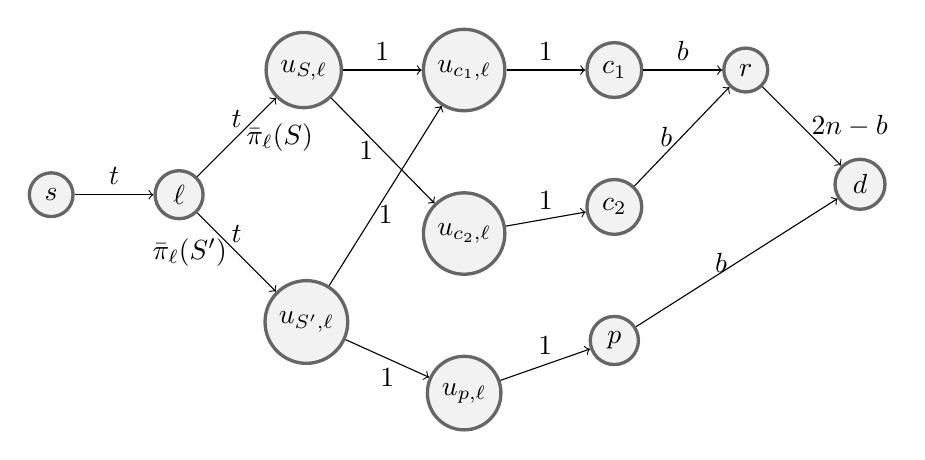
\begin{tikzpicture}[
mynode/.style={circle, draw=black!60, fill=black!5, very thick, minimum size=5mm},
]
\node[mynode](s){\normalsize $s$};
\node[mynode](ell)[right=of s]{\normalsize $\ell$};
\node[mynode](us1ell)[above right=of ell]{\normalsize  $u_{S,\ell}$};
\node[mynode](us2ell)[below right=of ell]{\normalsize $u_{S',\ell}$};
\node[mynode](uc1ell)[right=of us1ell]{\normalsize $u_{c_1,\ell}$};
\node[mynode](uc2ell)[below=of uc1ell]{\normalsize $u_{c_2,\ell}$};
\node[mynode](upell)[below=of uc2ell]{\normalsize $u_{p,\ell}$};
\node[mynode](c1)[right=of uc1ell]{\normalsize $c_1$};
\node[mynode](c2)[below=of c1]{\normalsize $c_2$};
\node[mynode](p)[below=of c2]{\normalsize $p$};
\node[mynode](r)[right=of c1]{\normalsize $r$};
\node[mynode](d)[below right=of r]{\normalsize $d$};
\draw[->](s) -- (ell) node [midway, above] {\normalsize $t$};
\draw[->](ell) -- (us1ell) node [midway, above] {\normalsize $t$} node [midway, right] {\normalsize $\bar{\pi}_{\ell}(S)$} ;
\draw[->](ell) -- (us2ell) node [midway, above] {\normalsize $t$} node [midway, left] {\normalsize $\bar{\pi}_{\ell}(S')$} ;
\draw[->](us1ell) -- (uc1ell) node [midway, above] {\normalsize $1$};
\draw[->](us1ell) -- (uc2ell) node [midway, left] {\normalsize $1$};
\draw[->](us2ell) -- (uc1ell) node [midway, below] {\normalsize $1$};
\draw[->](us2ell) -- (upell) node [midway, below] {\normalsize $1$};
\draw[->](uc1ell) -- (c1) node [midway, above] {\normalsize $1$};
\draw[->](uc2ell) -- (c2) node [midway, above] {\normalsize $1$};
\draw[->](upell) -- (p) node [midway, above] {\normalsize $1$};
\draw[->](c1) -- (r) node [midway, above] {\normalsize $b$};
\draw[->](c2) -- (r) node [midway, left] {\normalsize $b$};
\draw[->](r) -- (d) node [midway, right] {\normalsize $2n-b$};
\draw[->](p) -- (d) node [midway, left] {\normalsize $b$};
\end{tikzpicture}
}
\caption{A sub-graph of $G(b)$ for $2$-approval. Assume that $S=\set{c_1,c_2}$ and $S'=\set{c_1,p}$. Edge labels are their capacity. Where edges have a second label, it is their cost. All other edge costs are zero.}
\label{flowExample}
\end{figure}
For any set $S \in \binom{C}{t}$, we let $\bar{\pi}_{\ell}(S)=\max_{c \in S}v_\ell(c)-t$.
We can assume w.l.o.g.\ that we know the value $b$, the final score of $p$ in the optimal demotion strategy (since we can try all the possible values for $b$ and choose the one resulting in the cheapest final solution).
We shall construct a priced flow network $G(b)$ in which units of flow represent awarded points, as follows. The vertex set  $U = \set{s,d,r} \cup N \cup U_1 \cup U_2 \cup C$ is comprised of the following `layers' (visualized in \cref{flowExample}).
\begin{itemize}
    \item $N$ (resp.\ $C$) represents the voter set (resp.\ candidate set); a flow unit passing through a vertex $\ell \in N$ (resp.\ $c \in C$) represents a point awarded by $\ell$ (resp. awarded to $c$).
    \item $U_1 = \setgiven{u_{S,\ell} \given S \in \binom{C}{t}, \ell \in N}$; a flow unit passing through a vertex $u_{S,\ell} \in U_1$ represents a point awarded by $\ell$ to a candidate in $S$ (the choice of \emph{which candidate} will be immediately discussed).
    \item $U_2 = \setgiven{u_{c,\ell} \given c \in C, \ell \in N} \in U_2$; a flow unit passing through a vertex $u_{c,\ell}$ represents a point awarded by $\ell$ to the candidate $c$.
    \item $s$ and $d$ are the \emph{source} and \emph{destination} vertices. $r$ represents any candidate other than $p$.
\end{itemize}
The edge set $E=E_1 \cup E_2 \cup E_3 \cup E_4 \cup E_5 \cup E_6$ is comprised of the following, where $\gamma(u,v)$ is the capacity of an edge $(u,v)$ and  $a(u,v)$ is its cost.
\begin{itemize}
    \item $E_1=\setgiven{(s,\ell) \given \ell \in N}$ with all capacities equal to $t$, guarantees that each voter has at most $t$ points to distribute.
    \item $E_2= \setgiven{(\ell, u_{S,\ell})\given \ell \in N, S \in \binom{C}{t}}$ with capacities equal to $t$, will be discussed later.
    \item $E_3=\setgiven{(u_{S,\ell}, u_{c,\ell})\given \ell \in N, c \in S}$ with all capacities equal to $1$, guarantees that each candidate can receive at most one point from a subset he is a member of.
    \item $E_4= \setgiven{(u_{c,\ell},c) \given c \in C, \ell \in N}$ with all capacities equal to $1$, guarantees that each candidate can receive at most one point from a specific voter.
    \item $E_5= \setgiven{(c,r) \given c \in \Cmp}$, with all capacities equal to $b$ guarantees that each candidate will receive at most $b$ points (where $b$ will be $p$'s final score).
    \item $E_6= \set{(p,d),(r,d)}$, where $\gamma(p,d)=b$ and $\gamma(r,d)=tn-b$. By later setting the desired flow value to $tn$, these edges will be saturated, and $p$'s score will be exactly $b$.
\end{itemize}
For each edge $(\ell, u_{S,\ell}) \in E_2$, we let $a(\ell, u_{S,\ell}) = \bar{\pi}_{\ell}(S)$. All other edge costs are $0$. Finally we let $G(b)=(U,E,\gamma,a)$. An example of a sub-graph of $G(b)$ is shown in \cref{flowExample}.
The main procedure is the following. Given $b$, construct $G(b)$, and run a \CMCF{} algorithm on it with a desired flow value $tn$ \cite{edmonds1972theoretical}. If it failed to find such a flow then return a \emph{fail} status; otherwise, denote the resulting network flow as $f$. We shall modify $f$ to become another flow $f'$ as follows.
For each voter $\ell$, let $S'_{\ell} = \setgiven{c \given f(u_{c,\ell},c)=1}$. We will prove that $\abs{S'_{\ell}}=t$. We define $f'(\ell, u_{S'_{\ell},\ell})=t$, $f'(u_{S'_{\ell},\ell}, u_{c,\ell})=\indic_{S'_{\ell}}(c)$, $f'(\ell,u_{S,\ell})=0$ for all $S \neq S'_{\ell}$, and $f'(u_{S,\ell}, u_{c,\ell})=0$ for all $S \neq S'_{\ell}$.
Based on $f'$, we compute the following demotion strategy $Q$:  perform the necessary demotions such that for each $\ell$, the candidates in $S'_{\ell}$ become the top $t$ candidates in $v_\ell$; this is done by demoting all candidates $c' \notin S'_{\ell}$ for which $v_\ell(c') < \max_{c \in S'_{\ell}} v_\ell(c)$ to the bottom of $v_\ell$.
Our approximation algorithm, denoted $\mathcal{M}$, repeats the above procedure for each $b \in [n]$, and returns the strategy $Q$ having the minimum cost out of all strategies computed.
Let $Q^{\star}$ be the optimal demotion strategy. In the following lemmas, we will argue that the above algorithm returns a demotion strategy $Q$ for which $\pi(Q) \leq t\pi(Q^{\star})$.
\begin{lemma} \label{edgesCostsLemma}
For a size-$t$ set $S$, the minimal price for making all the candidate in $S$ become the top $t$ candidates in $v_\ell$ is $\bar{\pi}_{\ell}(S)=\max_{c \in S}v_\ell(c)-t$.
\end{lemma}
\begin{proof}
Let $c' = \argmax_{c \in S}v_\ell(c)$ be the bottom-most candidate in $S$ w.r.t.\ $v_{\ell}$. The number of candidates not in $S$ who are ranked before him in $v_\ell$ is exactly $v_\ell(c')-t$.
\end{proof}
Let $b^\star$ be the final score of $p$ under  $Q^\star$.
\begin{lemma}\label{flowIsMaximal}
There exists a potential flow $f^\star$ in $G(b^\star)$ where $\abs{f^\star} = tn$ and $\Aoper{f^\star} = t\cdot \pi(Q^\star)$.
\end{lemma}
\begin{proof}
 We define $f^\star$ in $G(b^\star)$ as follows. For each $\ell$, let $S^\star_\ell$ be the candidates $\ell$ approves of following the demotion operations in $Q^\star$, and let $s^\star(c)$ be the resulting score of $c$. Set $f^\star(\ell, u_{S^\star_\ell,\ell}) = t$, $f^\star(u_{S^\star_\ell,\ell}$, $u_{c,\ell}) = \indic_{S^\star_{\ell}}(c)$, $f^\star(u_{c,\ell},c) = \indic_{S^\star_{\ell}}(c)$, $f^\star(c,r) = s^\star(c)$, $f^\star(r,d)=\sum_{c \in \Cmp}s^\star(c)=tn-b^\star$,  $f(p,d)=b^\star$. All other edges will have $0$ flow. It can be easily verified that all the flow conditions are satisfied, that $\abs{f^\star} = f(r,d)+f(p,d) = tn$, and that $\Aoper{f^\star} =  \sum_{\ell}a(\ell, u_{S^\star_\ell, \ell})f^\star(\ell, u_{S^\star_\ell, \ell})= t \cdot \sum_{\ell}a(\ell, u_{S^\star_\ell, \ell}) =  t \cdot \sum_{\ell}\bar{\pi}_{\ell}(S^\star_\ell)= t\cdot \pi(Q^\star)$.
\end{proof}
The following lemmas assume that the algorithm did not fail on $G(b)$, and thus $\abs{f} = tn$.
\begin{lemma}
For each voter $\ell$, $\abs{S'_\ell}=t$. $f'$ is well-defined, is a valid flow, and  $\abs{f'} = tn$.
\end{lemma}
\begin{proof}
We have that $\abs{f} = tn$. As every voter $\ell$ has an incoming capacity of $t$, each voter transfers exactly $t$ flow units to candidates.
Fix a voter $\ell$. Since $\gamma(u_{c,\ell},c) = 1$ for each $c$, there must be exactly $t$ candidates
such that each receives a unit flow from $\ell$. Therefore $\abs{S'_\ell}=t$ and $u_{S'_\ell, \ell}$ is a node in $G(b)$. When defining $f'$, after identifying the set $S'_\ell$, the algorithm simply reroutes the $t$ flow units to the the candidates in $S'_\ell$ through $u_{S'_\ell, \ell}$, thus the flow value is maintained.
\end{proof}
\begin{lemma} \label{totalPriceLemma}
It holds that $\Aoper{f'} \leq t \cdot \Aoper{f}$.
\end{lemma}
\begin{proof}
Fix a voter $\ell$, and let $R=\setgiven{S \given  f(\ell, u_{S, \ell})\geq 1}$. Now consider the candidate set $C' = \bigcup_{S \in R}S$ and the set $S_{\max}=\argmax_{S\in R} \bar{\pi}_{\ell}(S)$. Let $c'$ be the candidate $c \in C'$ maximizing $v_\ell(c)$ and notice that $c' \in S_{\max}$. Now consider $S'_{\ell}$ as defined by the algorithm and notice that $S'_{\ell} \subseteq C'$ by the flow properties: a unit of flow which reaches a candidate $c$ from $\ell$ must pass through some node $u_{S,\ell}$ such that $c \in S$. Therefore---applying \Cref{edgesCostsLemma}---$\bar{\pi}_{\ell}(S') \leq \bar{\pi}_{\ell}(S_{\max})$.
It follows that $a(\ell, u_{S'_\ell, \ell})f'(\ell, u_{S'_\ell, \ell}) =t \cdot a(\ell, u_{S'_\ell, \ell})  \leq t\cdot  a(\ell, u_{S_{\max}, \ell}) \leq
t\cdot \sum_{S \in R}a(\ell, u_{S, \ell}) f(\ell, u_{S, \ell})$.
The lemma follows by summing the last inequality over all voters $\ell \in N$, and recalling that for each edge $e \notin E_2$, $a(e)=0$.
\end{proof}
\begin{theorem}
Algorithm $\mathcal{M}$ returns a valid solution $Q$ making $p$ win, and $\pi(Q) \leq t \pi(Q^{\star})$.
\end{theorem}
\begin{proof}
It is enough to show that in the iteration where $b = b^{\star}$, we find a solution  $Q' $ such that $\pi(Q' ) \leq t \pi(Q^{\star})$.
As proven in \Cref{flowIsMaximal}, when $b = b^{\star}$ there exists a maximal flow $tn$ in $G(b^{\star})$ and therefore our algorithm will find such a flow. Consider $f$ and $f'$, the min-cost flow and the constructed flow in this iteration. Also consider  $f^\star$, the flow induced by the optimal strategy as detailed in \Cref{flowIsMaximal}.
It holds that $\abs{f'} = tn$ and $\Aoper{f'} \leq t \cdot \Aoper{f} \leq t \cdot \Aoper{f^\star} $. Since $\abs{f'} = tn$, then $f'(p,d)=b$. Since $f'(c,r)\leq b$ for all $c \in \Cmp$, $p$ is necessarily winning.
For the flow $f'$,  it holds that
\begin{align*}
    \Aoper{f'} &= \sum_{\ell \in N}a(\ell, u_{S'_\ell, \ell})f'(\ell, u_{S'_\ell, \ell})\\
    &= t \cdot \sum_{\ell \in N}a(\ell, u_{S'_\ell, \ell})\\
    &=  t \cdot \sum_{\ell \in N}\bar{\pi}_{\ell}(S'_\ell)\\
    &= t\cdot \pi(Q')\ .
\end{align*}
We obtain that $\pi(Q') = \Aoper{f'}/t \leq  \Aoper{f^\star} = t \cdot \pi(Q^\star)$, where the inequality follows from \Cref{totalPriceLemma} and the final equality from \Cref{flowIsMaximal}.
\end{proof}
We make two important remarks: (a) our algorithm can be easily extended to support prices that are a function of the voters (by re-defining $a(\ell, u_{S,\ell})$ to be also multiplied by the voter's price); and (b) our algorithm provides an exact solution in the specific case of Plurality (as $t=1$).
\section{Borda}
In this section we will show $\NP$-hardness and a $3$-multiplicative approximation for Borda.
\subsection{\boldmath{$\NP$}-Hardness}\label{sec:borda_hardness}
\begin{theorem}\label{thr:borda_hardness}
Given a value $k$, determining whether there exists a solution to Borda-\SB{} with at most $k$ demotions  is $\NP$-hard.
\end{theorem}
\begin{proof}
Given an instance $I=(U,\mathcal{S})$ of \SC{} and a desired cover size $k \leq \bar{m}$, we define a reduction as follows.
We define the candidate set $C=U \cup  D \cup \set{p,a,b}$, where $D=\set{d_0,\ldots,d_{\bar{n}-2}}$ is a set of $\bar{n}-1$ dummy candidates, $p$ is the preferred candidate and $a,b$ are  two additional candidates. We let $D_{<q}=\set{d_0,\ldots,d_{q-1}}$ and $D_{\geq q}=\set{d_{q},\ldots,d_{\bar{n}-2}}$.
The preference profile is defined as follows. For each set $S_i \in \mathcal{S}$, we define two preference orders $v_i^1,v_i^2$, such that
\begin{align}
    v_i^1 &= \ora{D_{\geq \abs{S_i}}} \succ  \ora{S_i}  \succ  a \succ b \succ \ora{U \setminus S_i}\succ \ora{D_{<\abs{S_i}}} \succ p   \\
    v_i^2 &=  p  \succ \ola{D_{<\abs{S_i}}} \succ \ola{U \setminus S_i} \succ b \succ a \succ \ola{S_i} \succ  \ola{D_{\geq \abs{S_i}}}\ .
\end{align}
In addition, we define the following two preference orders:
\begin{align}
    \bar{v} &=  \ora{D} \succ a \succ b \succ  \ora{U}  \succ p \\
    \hat{v} &=  p \succ \ola{U}  \succ a \succ b \succ \ola{D} \ .
\end{align}
Finally, we define the following two preference orders:
\begin{align}
    \bar{v}' &= \ora{D} \succ a \succ \ora{U} \succ b  \succ p  \\
    \hat{v}' &=  p \succ \ola{U}  \succ a \succ b \succ \ola{D}\ .
\end{align}
We let
$$V=\set{v_i^1,v_i^2}_{i=1}^{\bar{m}} \cup \set{\bar{v}_j, \hat{v}_j}_{j=1}^{k(\bar{n}+3)-1} \cup \set{\bar{v}', \hat{v}'}\ ,$$
where each $\bar{v}_j$ (resp.\  $\hat{v}_j$) is a copy of $\bar{v}$ (resp.\  $\hat{v}$).\footnote{While $V$ is a list of preference orders, with a slight abuse of notation, we have defined it using set operations.} Let $E = (C,V)$ be the resulting election.
\begin{lemma}
For $E$, it holds that  $\diff(a,p)=k(\bar{n}+3)$,  that $\diff(p,b)= k(\bar{n}+3) + \bar{n}$, and that
  $\diff(p,d)= 0$  for every $d \in D$. In addition, $\diff(u_1,p)=\cdots=\diff(u_{\bar{n}},p)=1$.
\end{lemma}
By summing the points awarded to each candidate. To see that more easily, notice that each pair of preference orders defined above awards $m-1$ points to each candidate, unless the following event occurs: whenever $c \succ c'$ in \emph{both} of the pair's preference orders, it effectively means that a points is `transferred' from $c'$ to $c$.
\begin{lemma}\label{lem:pushed}
Let $Q$ be a winning demotion strategy for $E$ with $k$ demotion operations. Then all bribed voters have votes of types $v_i^1$, $\bar{v}$, or $\bar{v}'$, and in each of them  $a$ was demoted by $\bar{n}+2$ positions.
\end{lemma}
\begin{proof}
Let $s(c)$ be the score of candidate $c$ after the demotion operations.
Since we have $k$ demotion operations, $s(p)$ will be at most $\sigma(p)+k$. To make $p$ indeed win we require that $s(a) \leq s(p)$, thus $a$ should lose \emph{at least} $k(\bar{n}+2)$ points. However, notice that for each voter, $a$ can be pushed down at most $\bar{n}+2$ positions. Indeed, only for voters of types $v_i^1, \bar{v}, \bar{v}'$, $a$ can be demoted by $\bar{n}+2$ positions (for all other voters, $a$ can be demoted by at most $\bar{n}+1$ positions). Thus, to reach the desired decrease in score, only voters of types $v_i^1, \bar{v}, \bar{v}'$ can be bribed, each once, and in each operation  $a$ will be demoted exactly $\bar{n}+2$ positions. As a result, $s(a)=s(p)=\sigma(p)+k$.
    \end{proof}
We are now ready to complete the proof of \Cref{thr:borda_hardness} by showing that
$E$ has a winning strategy with $k$ operations if and only if $U$ can be covered by $k$ subsets of $\mathcal{S}$.
\textit{Completeness:} Let $\mathcal{S}'$ be a valid $k$-cover. For each $S_i \in \mathcal{S}'$, bribe $v_i^1$ and move $a$ to the last position in $v_\ell$. Notice that now $s(p) =s(a) = \sigma(p)+k$. Now focus on the effect of bribing a single voter $v_i^1$:  it does not change the value $\diff(p,u)$ for each $u \in U\setminus S_i$, but increases $\diff(p,u)$ by $1$ for each $u \in S_i$. Since $\mathcal{S}'$  is a proper cover, it means that according to our scheme, for each $u$ there exists at least one bribed voter $v_i^1$  who  increases $\diff(p,u)$ by $1$ (this is a voter $v_i^1$ for which $S_i \in \mathcal{S}'$ and $u \in S_i$), thus at the end of the bribery process, $\diff(p,u) \geq 0$. We have just showed that $s(p) \geq s(u)$ for each $u \in U$, and that $s(p) \geq s(a)$. As for the remaining candidates in $D \cup \set{b}$, notice that at first they were ranked equally or less than $p$, and that each time one of them was promoted, $p$ was promoted as well, and therefore $\diff(p,c)$ does not decrease for each $c \in D \cup \set{b}$. We conclude that as a result of this bribery scheme, $p$ now wins.
\textit{Soundness:} Assume that $p$ can be made to win by bribing $k$ voters, and consider the corresponding demotion strategy. By \Cref{lem:pushed}, in all bribed votes  $a$ was pushed down $\bar{n}+2$ positions. Now observe only the bribed voters of type $v_i^1$. Since  for each $u \in U$ it held before that $\diff(p, u) = -1$, but now $\diff(p, u) \geq 0$, we bribed at least one voter $v_i^1$ such that $u \in S_i$, which allowed $\diff(p, u)$ to increase by a point. Therefore, the collection $\mathcal{S}' = \setgiven{S_i \in \mathcal{S} \given v_i^1 \text{ is bribed}}$ constitutes a valid cover. Since $\abs{\mathcal{S}'} \leq k$
we are done.
\end{proof}
\subsection{Approximation}
The main idea behind our approximation is noticing that the hardness of \SB{} under Borda stems from the fact that when we demote a candidate by $\delta$ positions, then $\delta$ candidates receive a point. Now assume that we ignore this issue for a moment. This is equivalent to  range voting (RV) where each voter awards a score between $0$ and $m-1$ to each candidate. Here, demoting a candidate---e.g., by having a voter decrease her awarded score by $\delta$ points---does not have any consequence on the score of other candidates.
\begin{algorithm}[tb]
\caption{$\CF((C,\bar{V}), k, T)$ \label{ConsequenceFreeAlg}}
\SetKwInOut{Input}{input}
\SetKw{Break}{break}
\SetKw{Fail}{fail}
$Q \gets \varnothing$\;
\ForEach{$c \in C$}{
$S_{c} \gets \setgiven{ (\ell, \delta) \given (c, \delta) \in \bar{v}_{\ell},\ \ell=1,\ldots,n }$\;
$s_c \gets \sigma(c)$\;
}
\For{$i\gets 1$ \KwTo $k$}{
$C' \gets \setgiven{c \in C \given s_c > T}$\;
\If{$C' = \varnothing$}{\Break}
Pick an arbitrary  $c \in C'$.\;
 $(\ell',\delta') \gets \argmax_{(\ell,\delta) \in S_c}\delta$\;
$Q \gets Q \cup \set{(\ell', c, \delta')}$\;
$S_{c} \gets S_{c} \setminus \set{(\ell',\delta') } $\;
$s_c \gets s_c - \delta'$\;
}
$C' \gets \setgiven{c \in C \given s_c > T}$\;
\leIf{$C' = \varnothing$}{\Return $Q$\label{ConsequenceFreeAlg:returnB}
}{\Fail}
\end{algorithm}
We  start by reducing our instance into a corresponding RV instance $\bar{E}$: we naturally translate a ranking in the $j$-th place of a candidate by a voter to awarding him a score of $\alpha_j=m-j$ by the voter.
In the reduced instance, we look for the smallest $k$ for which we can make sure---using at most $k$ demotion operations---that all candidate scores do not exceed a bound $T = \sigma(p) + k$. We refer to \SB{} under RV with this goal as \emph{bounded} \SB{} under RV.
We denote the function that---given a RV instance, and the values $k$ and $T$---either returns a sequence of at most $k$ demotion operations or fails---as $\CF(\bar{E}, k, T)$.
Computing $\CF{}$ is easily achievable by a greedy algorithm which iteratively: (a)  identifies a \emph{violating candidate} for which the score exceeds $T$; (b) finds the voter who awards him the maximal number of points; and (c) performs a demotion operation, decreasing the score given by this voter to the candidate to $0$. The algorithm for $\CF$ is illustrated as \Cref{ConsequenceFreeAlg}.
After finding the smallest $k$ for which $\CF(\bar{E}, k, \sigma(p) + k)$ succeeds, we take the resulting demotion strategy and apply it on the original Borda instance. Unfortunately, these operations now do have their consequences, and candidate scores might increase as a result of the demotion operations. However, we will prove that not by too much. In any case, $p$ might be losing. We address this by repeating the following procedure: we  find a voter who currently has $p$ at any position but the top one, and then swap $p$ and the candidate ranked above him by this voter. We shall repeat this step until $p$ is winning. The overall algorithm is described in \Cref{3k-approxAlg}.
\begin{algorithm}[tb]
\caption{\SB{} for Borda}
\label{3k-approxAlg}
\SetKwInOut{Input}{input}
\SetKw{Break}{break}
\SetKw{Continue}{continue}
\SetKw{Fail}{fail}
$\bar{V}=( \bar{v}_{\ell})_{\ell}$ where $\bar{v}_{\ell} = \setgiven{(c, \alpha_{v_\ell(c)})\given c \in C \setminus \set{p}}$\;
Let $\bar{E} = (C \setminus \set{p}, \bar{V})$\label{line:construct}\;
Let $k'$ be the minimum $k$ for which $\CF(\bar{E}, k, \sigma(p)+k)$ does not fail\label{3k-approxAlg:t-definition}\;
$Q \gets \CF(\bar{E}, k', \sigma(p)+k')$ \label{3k-approxAlg:BeforeBribe}\;
\ForEach{$(\ell, c, \delta) \in Q$ \label{3k-approxAlg:ConFreeBribes}}{
Demote $c$ in $v_{\ell}$ by $\delta$ positions.\;
}
\While{$p$ is not winning \label{3k-approxAlg:ReparePLoop}}{
Let $\ell \in N, c \in C \setminus \set{p}$  such that $c$ is ranked immediately before $p$ in $v_{\ell}$.\;
Demote $c$ in $v_{\ell}$ by one position.
}
\Return the sequence of demotion operations performed.\;
\end{algorithm}
\begin{lemma}
\Cref{ConsequenceFreeAlg} finds a solution to bounded \SB{} under range voting ($\CF$).
\end{lemma}
\begin{proof}
For RV, a demotion of a candidate by a voter does not have any consequences on other voters and candidates. Therefore, a simple greedy procedure of repeatedly identifying and demoting a violating candidate is sufficient. \end{proof}
\begin{lemma}\label{lem:corresponding}
Let $E$ be a preferential election under Borda, and let $\bar{E}$ be its corresponding election under RV, as constructed in \Cref{line:construct} of \Cref{3k-approxAlg}. Then:
\begin{itemize}
    \item A sequence of operations $Q$ for range voting can be applied on the Borda instance, only that in each operation $(\ell, c, \delta) \in Q$, $\delta$ now pertains to the number of positions $c$ is demoted by in $v_\ell$ (for  RV $\delta$ was the decrease in points).
    \item A sequence of operations $Q$ applicable on $E$ can be modified into a sequence of operations $f(Q)$  applicable on $\bar{E}$ such that the final score of each candidate in the RV setting will be at most his final score in the Borda setting.
\end{itemize}
\end{lemma}
\begin{proof}
For the first item, assume that we apply each operation in $Q$ sequentially, in parallel on the two elections. In Borda, an operation $(\ell, c, \delta)$ might have side effects on other candidates, however the value $v_{\ell}(c')$ for any  candidate $c' \neq c$ can only decrease. As such, if a later applied operation is of the type $(\ell, c' ,\delta')$, this means that the score currently awarded to $c'$ by $\ell$ in the Borda instance is at least $\delta'$, and thus $c'$'s rank is at most $m-\delta'$, meaning that the operation can be safely applied.
For the second item, simply replace each  operation $(\ell, c, \delta) \in Q$ with an operation $(\ell,c,\delta')$ where $\delta'$ is the score currently awarded to $c$ by $\ell$ in the RV instance (so that following the operation, the score  awarded to $c$ by $\ell$ is $0$).
\end{proof}
Let $k^{\star}$  be the optimal number of demotion operations required to make $p$ win, and let $k'$ be the value from \Cref{3k-approxAlg:t-definition} of \Cref{3k-approxAlg}.
\begin{lemma} \label{k-star-consequenceFreeLemma}
$\CF(\bar{E},k^{\star},\sigma(p)+k^{\star})$ does not fail. In particular, this implies that $k' \leq k^{\star}$.
\end{lemma}
\begin{proof}
For \SB{} under Borda, if $p$ can be made to win by at most $k^\star$ demotion operations, then $p$'s final score $s(p)$ is at most $\sigma(p)+k^\star$. In addition, following these operations, each other candidate score is at most $s(p) \leq \sigma(p)+k^\star$. Let $Q^\star$ be the demotion strategy applied by an optimal strategy on $E$. Assume we apply the strategy $f(Q^\star)$ as defined by \Cref{lem:corresponding} on $\bar{E}$. Since here when we demote a candidate, other candidate scores do not increase, each candidate's final score is at most his corresponding Borda final score. As such, the sequence $f(Q^\star)$ is a valid solution for $\CF(\bar{E},k^{\star},\sigma(p)+k^{\star})$.
\end{proof}
\begin{lemma} \label{2t-loopLemma}
The loop in \Cref{3k-approxAlg:ReparePLoop} of \Cref{3k-approxAlg} will run at most $2k'$ times.
\end{lemma}
\begin{proof}
Let $s'(c)$ be the score of a candidate $c$ right before \Cref{3k-approxAlg:ReparePLoop} of \Cref{3k-approxAlg}.
The demotion strategy $Q$  found in \Cref{3k-approxAlg} guarantees that under RV, each candidate's score will be at most $\sigma(p)+k'$. In contrast, when applying $Q$ on the original Borda instance $E$ (which is possible by \Cref{lem:corresponding}), each candidate might be awarded one additional point for each operation. As $\pi(Q) \leq k'$, this means that the score of each candidate might increase by additional $k'$ points compared to their final RV score. Thus $s'(c) \leq \sigma(p) + 2k'$ for each $c \in C \setminus \set{p}$.
As $s'(p) \geq \sigma(p)$, at most $2k'$ swaps promoting $p$ are enough to make him win.
\end{proof}
\begin{theorem}
\Cref{3k-approxAlg} is a $3$-approximation algorithm for \SB{} under Borda.
\end{theorem}
\begin{proof}
As $k' \leq k^\star$ (by \Cref{k-star-consequenceFreeLemma}), it is sufficient to show that \Cref{3k-approxAlg} performs at most $3k'$  operations. To see that, notice that $\pi(Q) \leq k'$ and that the loop of \Cref{3k-approxAlg:ReparePLoop} of \Cref{3k-approxAlg} runs   at most $2k'$ times (by \Cref{2t-loopLemma}), where each iteration involves a single demotion operation.
\end{proof}
\subsection{Inapproximability Results \label{inaprox}}
What if the price of a demotion is a function of both the bribed voter and the demoted candidate? Indeed, assigning prices for different demographic-candidate pairs is consistent with the observation that the effect of negative campaigns changes with different  demographic and targeted candidate combinations. Some demographics were shown to be more tolerant to negativity in campaigns, while others might pose a risk for a backlash against the favored candidate. In addition, the effectiveness of such attacks was shown to be dependent on candidate properties, such as ethnicity, gender, and whether the candidate is  incumbent or challenging \cite{fridkin2011variability}.
Interestingly enough, when the price function is of type $\hat{\pi}\colon N \times C \to \preals$  ($\hat{\pi}(\ell,c)$ is the price for demoting $c$ in $v_\ell$), \SB{} for Borda is hard to approximate within some ratio:
\begin{theorem}
With the price function $\hat{\pi}\colon N \times C \to \preals$, for every constant $\epsilon >0$, \SB{} for Borda cannot be approximated within $(1-\epsilon) \ln (m/2-1)$ in polynomial time unless $\Pclass = \NP$.
\end{theorem}
\begin{proof}
Let $f$ be the reduction from \SC{} described in the proof of  \Cref{thr:borda_hardness}, adjusted such that in $f(I,k)$,  for each voter $\ell$ with a vote in $\set{v_i^1}_{i=1}^{\bar{m}}$,  $\pi(\ell,a) = 1$ and $\pi(\ell,c) = k\ln (m/2-1)$ for every $c \neq a$. In addition, every voter $\ell$ with vote in $V \setminus \set{v_i^1}_{i=1}^{\bar{m}}$,  $\pi(\ell,c) = k\ln (m/2-1)$ for every $c \in C$.
Assume by contradiction that there exists a polynomial-time $(1-\epsilon) \ln (m/2-1)$-approximation algorithm $\mathcal{A}$ for \SB{} with prices $\hat{\pi}$.
Assume that we know what is the optimal set cover size $k$.
In this case, we know that a strategy of price $k$ exists, by an argument very similar to the completeness argument in \Cref{thr:borda_hardness}. % TODO(avishai): Verify this lemma.
In this case, $\mathcal{A}(f(I,k))$ will find a strategy of price of at most $(1-\epsilon) k \ln (m/2-1)$ in polynomial time.
Now focus on the strategy returned by $\mathcal{A}(f(I,k))$. By the overall price paid being at most  $ (1-\epsilon) k\ln (m/2-1)$, we know that only voters having votes of type $v_i^1$ were bribed, and that in each such operation, $a$ was demoted. We can assume w.l.o.g.\ that in each operation, $a$ was demoted  to be ranked last, otherwise we can modify the operation so that this will be the case; although this modification might award a point to some additional candidates, since it will also award an additional point to $p$, then $\diff(p,c)$ for any $c \in C$ can only maintain its value or increase. Specifically, after applying these modifications $p$ is still winning and no price increase was made.
We again reach a point where for all bribed voters  $a$ was pushed down $\bar{n}+2$ positions. Now observe only the bribed voters having votes of type $v_i^1$. Since  for each $u \in U$ it held before that $\diff(p, u) = -1$, but now $\diff(p, u) \geq 0$, we bribed at least one voter having a vote of type $v_i^1$ such that $u \in S_i$, which allowed $\diff(p, u)$ to increase by a point. Therefore, the collection $\mathcal{S}'' = \setgiven{S_i \in \mathcal{S} \given v_i^1 \text{ is bribed in } \mathcal{A}(f(I,k))}$ constitutes a valid cover and  $\abs{\mathcal{S}''} \leq (1-\epsilon) k \ln (m/2-1) = (1-\epsilon) k \ln \bar{n}$.
We can now relax the assumption that we know what is the optimal set cover size $k$, by considering the following procedure for \SC{}: for $k=1,\ldots,\bar{n}$, we compute $f(I,k)$ and apply  $\mathcal{A}$ on the result. If the returned strategy involved price at most  $ (1-\epsilon) k\ln (m/2-1)$, halt and extract the set cover from the bribery strategy as described above. Notice that this procedure will have to halt and succeed at the iteration where $k$ is indeed the optimal set cover size (if not even before). The procedure we have just described is a  $(1-\epsilon) \ln \bar{n}$-approximation to \SC{}.
However,  this contradicts the inapproximability of \SC{} within a $(1-\epsilon) \ln \bar{n}$ factor, unless $\Pclass = \NP$, as shown by Dinur and Steurer \shortcite{DBLP:conf/stoc/DinurS14}.
\end{proof}
\section{Destructive Variants}
For the destructive variant \DTNC{} our goal it to make the currently leading candidate $d \in C$ lose (by making sure he will not be in the winner set). To this end we introduce a polynomial algorithm for scoring rules, applicable even when voters have prices $\pi(\ell)$ for each voter $\ell$. We assume that  each score value of the scoring rule is representable as an $O(\log{(nm)})$-bit integer (notice that the `natural' input size is $\Theta(nm)$). This is a very natural assumption: it is trivially true for Plurality and Veto, $t$-approval, Borda and truncated variants thereof. Even Dowdall, for which $\alpha_j = 1/j$, can be modified to conform to this assumption, by noticing that the smallest difference between two score values in $\veca$ is at least $m^{-2}$. Thus, by rounding each score to the nearest multiple of e.g., $1/(2nm^2)$, a candidate's final score would change by at most $1/(2m^2)$ and the order induced by candidates' final scores will be unchanged. At this point, the modified scores can be normalized to become $O(\log{(nm)})$-bit integers. A scoring rule not satisfying our assumption is, for example, exponential-Borda \cite{DBLP:journals/tcci/PutF16}, for which $\veca=(2^{m-1},2^{m-2},\ldots,2^1,2^0)$.
It is sufficient that one candidate beats $d$, therefore, we can loop over each candidate $c$ and find the minimal-cost strategy making $c$ beat $d$.
Assume we do so, and let $c$ be such candidate. Let $Q^\star$ be the optimal strategy (unknown to us) making $c$ beat $d$. We can split $Q^\star$ to two sets of operations, $A$ and $B$, such that $A$ are all operations demoting $d$ and $B$ are all operation demoting a candidate other than $d$.
\begin{lemma}
W.l.o.g., all the following hold for $Q^\star$:
\begin{enumerate}
    \item All operations in $A$ were performed before all operations in $B$.
    \item All operations in $A$ demoted $d$ to be ranked last.
    \item All operations in $B$ involved demoting a candidate ranked immediately before $c$ to be immediately after $c$.
    \end{enumerate}
Let $\ell$ be a voter bribed during the execution of $B$, let $C'$ be the candidates demoted by $\ell$ within $B$, and let $t$ be the point in time following the operations in $A$ and before those of $B$.
    \begin{enumerate}
    \setcounter{enumi}{3}
    \item At time $t$, $c \succ_\ell d$.
    \item At time $t$, the candidates in $C'$ were ranked consecutively  immediately before $c$.
\end{enumerate}
\end{lemma}
\begin{proof}
The first three claims are straightforward. For the fourth claim,
assume that following the operations in $A$ it holds that $d \succ_{\ell} c$. $\ell$ was not bribed in $A$ because $d$ is above $c$. Let $c'$ be the voter demoted in this operation. Then we can demote $d$ instead of $c'$ and have an even greater effect on $\diff(d, c)$. However, in that case this operation can be placed as part of $A$. The fifth claim follows from the fact that if we demote $j$ candidates ranked before $c$, the choice of which  candidates is unimportant; in any case $c$ will gain $\alpha_{v_\ell(c) - j} - \alpha_{v_\ell(c)}$ points.
\end{proof}
Let $s$ be the change in $\diff(d,c)$ as a result of applying $A$, and notice that $0 \leq s \leq \diff(d,c) + \alpha_1 $ (in the edge-case where $B$ is empty, it is possible that the final operation in $A$ makes the change exceed $\diff(d,c)$). We do not know what $A$ is, but  we can exhaustively try all possibly values for $s$. Given the correct guess for $s$, we can then find $A$ using the following reduction to the $0$-$1$-Knapsack problem.
For each voter $\ell$ we create an  item $\ell$ with a  weight $w(\ell) = \pi(\ell)$ and a value $v(\ell) = (\alpha_{v_\ell(d)} - \alpha_m) + \indic{[d \succ_\ell c]} \cdot (\alpha_{v_\ell(c) - 1} - \alpha_{v_\ell(c)})$. This value represents the demotion of  $d$ to be last, such that $d$ loses $(\alpha_{v_\ell(d)} - \alpha_m)$ points and $c$ possibly gains $ (\alpha_{v_\ell(c) - 1} - \alpha_{v_\ell(c)})$ points (if $d$ was previously above him).
Our goal is to find the minimal total weight of items needed in order to obtain a value of at least $s$. Fortunately, Knapsack has an algorithm which is pseudo-polynomial in the values \cite{cormen2009introduction};\footnote{There is also an algorithm  pseudo-polynomial in the weights.} as our values can be represented as integers bounded by a polynomial in the input size, this Knapsack instance is polynomial-time solvable.
Once we have found $A$ for a guess of $s$, before we continue to finding $B$, we will require another  version of the Knapsack problem: let the sets $X_1,\ldots,X_n$ be a partition of a set of items, where each $X_\ell = \set{x_{\ell,1},\ldots,x_{\ell,\abs{X_\ell}}} $. Each such item has a weight $w(x_{\ell,j}) \geq 0$ and a value $v(x_{\ell, j}) \geq 0$.
Given a positive value $L$ the goal is to construct a set of items $S$ that minimizes $\sum_{x_{\ell,j} \in S}{w(x_{\ell,j})}$ while $\sum_{x_{\ell,j} \in S}{v(x_{\ell,j})} \geq L$, which also satisfies  the constraint that $\abs{S \cap X_\ell}\in\set{0,1}$ for each $\ell$.
This problem is a specific case of \textsc{Group Fairness Knapsack} (\CIK{}), studied by \citet{DBLP:journals/corr/abs-2006-07832}. For completeness, we provide an algorithm for our case in the following.
\begin{lemma}
\CIK{} can be solved in time polynomial in the input size and  pseudo-polynomial in $L$.
\end{lemma}
\begin{proof}
Let $f(k, i)$ represent the minimal weight needed in order to have a value of at least $k$ when only choosing from $X_1,\ldots,X_i$.
We can compute $f(L, n)$ (our objective) with dynamic programming using the following recursion:
$f(k, i) = \min_{0 \leq j \leq \abs{X_i}}(f(k - v(x_{i, j}), i - 1) + w(x_{i, j}))$ where $x_{i, 0}$ is a placeholder item  having zero weight and value representing not taking any item from the set. The edge cases are as follows:
$f(0, 0) = 0$; for every $k > 0 $,  $f(k, 0) = \infty$; and for each $k < 0, i \in [n]$, $ f(k, i) = 0$.
\end{proof}
We can now find $B$ (or an equivalent sequence of operations) by a reduction to \CIK{}:
For every voter $\ell$ create a set $X_\ell$ containing $v_\ell(c)-1$ items $x_{\ell,1},\ldots,x_{\ell,v_\ell(c) - 1}$, where for every $j \in [v_\ell(c) - 1]$ we define $w(x_{\ell, j}) = j \cdot \pi(\ell)$ and $v(x_{\ell, j}) = \alpha_{v_\ell(c) - j} - \alpha_{v_\ell(c)}$; the item $x_{\ell, j}$ represents the option of making $c$ gain $\alpha_{v_\ell(c) - j} - \alpha_{v_\ell(c)}$ points by demoting the $j$ candidates which are currently consecutively ranked immediately before $c$. We choose $L = \diff(d, c) - s + 1$ (i.e., $L$ is the difference between $d$ and $c$ after  the operations in $A$ were executed, plus an additional point to make sure that $d$ is not in the winner set).
\begin{theorem}
For every scoring rule, in which each score can be represented as an $O(\log{(nm)})$-bit integer, the \DTNC{} problem with prices which are a function of the voters can be solved in polynomial time.
\end{theorem}
\begin{proof}
Follows from the above discussion.
\end{proof}
\section{Conclusions}
The contribution of this work is twofold: first, we studied the de facto standard of political campaigns: targeted negative  campaigning. While being so widespread---as far as we know---it was not studied computationally. Second, our results show that it is a sweet-spot between \shiftB{}---which models positive campaigns---and \swapB{} which we feel is too granular: it models bribery and campaigning in a `local', swap-oriented level, instead of the more global effect or our demotion operations. As such our results for both the unpriced and priced variants are somewhere between the $(1+\epsilon)$ \shiftB{} approximation and the general inapproximability of \swapB{} for many voting rules.
We mention some directions for future research: (a) to better understand the complexity of  $t$-approval-\SB{} when $t=2$, or when $t$ is not fixed, and of Borda with a price  of the form $\pi\colon N \to \preals$; (b) to research other voting rules that are not necessary scoring rules, such as Copeland and Maximin.
Accusamus iste odio eos sed dolores voluptatibus possimus saepe, molestiae officiis expedita ipsa incidunt esse sit corrupti sed reprehenderit pariatur, expedita facere ut adipisci reiciendis odio, et cupiditate aliquid fugiat, id ut velit.Mollitia placeat accusamus sunt beatae earum veniam perferendis, dolorum neque modi voluptatibus dolore molestiae quae doloremque, est ipsum ea sed quibusdam vel voluptatibus eveniet qui, libero cum rem nam velit inventore deleniti ipsa voluptate earum mollitia asperiores, neque laborum libero ratione earum quos consectetur labore distinctio quibusdam.Dolore numquam possimus sit perspiciatis vel voluptate quaerat labore et eaque pariatur, asperiores obcaecati consectetur, repellendus recusandae quas aliquam nostrum nam explicabo, sint incidunt voluptatum quos eius nihil maxime assumenda sed, vitae enim vero consequuntur eligendi aliquid expedita mollitia?Eos recusandae fugiat quis architecto eius, aperiam voluptatum distinctio reprehenderit atque fugiat, nam delectus perferendis vel eveniet placeat libero, similique laudantium quas illum aut rem sed, qui eligendi placeat eos totam sit quae voluptatum?In tempora iste dolorem fugiat, aliquam maxime odit in doloribus perspiciatis quis ipsam, doloremque perspiciatis esse est fugiat sint inventore explicabo?Tenetur beatae sit nisi, eos veniam obcaecati, accusantium accusamus fuga quas vel, a maxime inventore deleniti nisi modi eos?\clearpage
\bibliography{main}
\end{document}